\subsubsection{Impact of Dual-Task Learning}
\label{sec:dual-task-result}


\begin{figure}[thbp]
\begin{center}
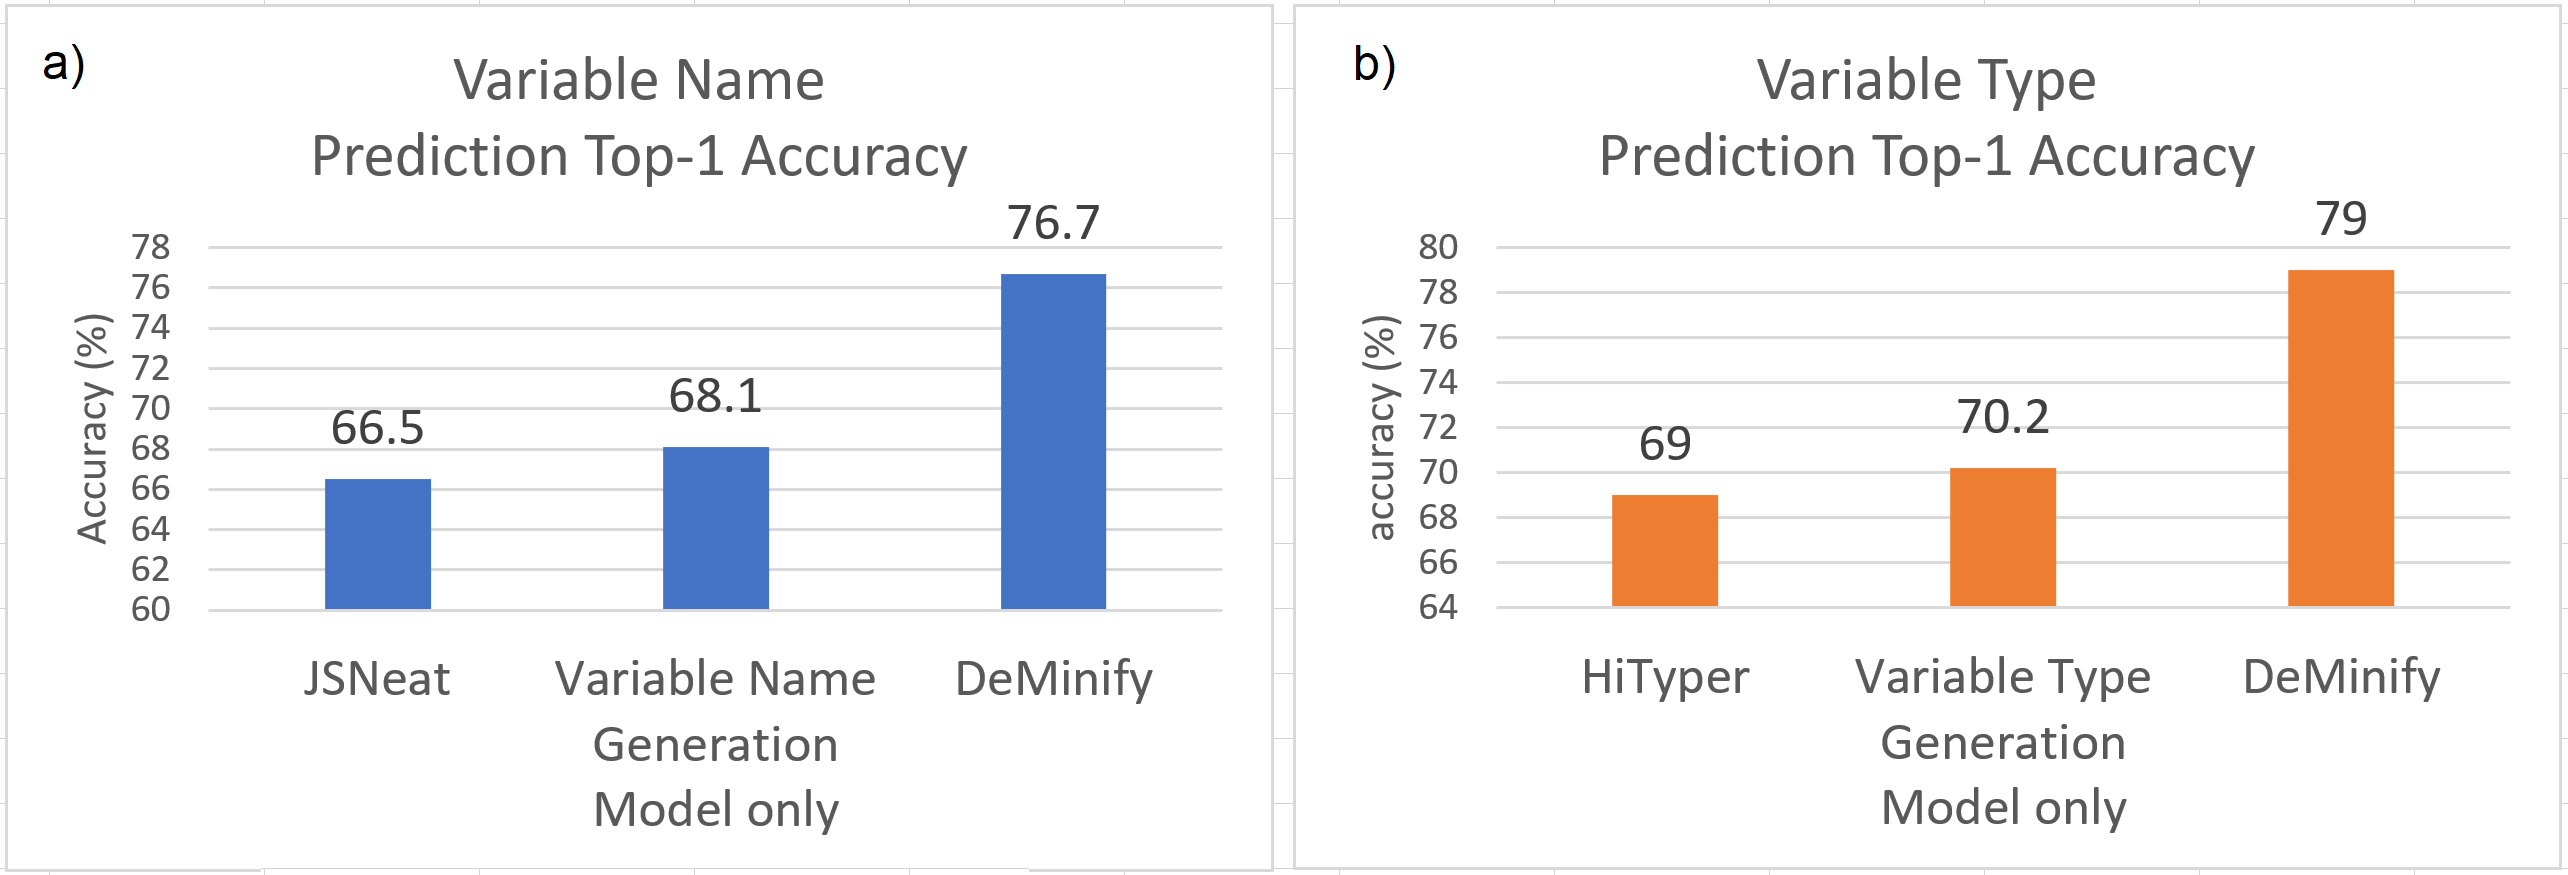
\includegraphics[width=3.4in]{figures/dual-task-result}
\vspace{-8pt}
\caption{RQ3. Impact of Dual-Task Learning}
\label{dual-task-result}
\end{center}
\end{figure}

Figure~\ref{dual-task-result}a) shows the Top-1 accuracy in variable
name prediction when we removed the dual-task learning scheme and
measured only the accuracy of the variable name generation (VNG)
model.  As seen, without the impact from variable type generation
(VTG) via dual-task learning, VNG performs only slightly better than
the best baseline, JSNeat (68.1\% versus 66.5\%). The drop in Top-1
accuracy from {\tool} is 12.6\% (from 76.7\% downto
68.1\%). Similarly, as seen in Figure~\ref{dual-task-result}b),
without the impact from VNG due to the removal of the dual-task
learning scheme, VTG performs about the same as the best baseline
HiTyper. The drop in Top-1 accuracy from {\tool} is 12.5\%.
These results indicate the positive contribution from our key idea
on the mutual impact of VNG and VTG via dual-task learning.
